%=====================================================================
\section{Lecture 2: The model, its bath, and the two kernels}
\label{sec:lec2}

\subsection{The Hamiltonian and its two faces}

The running model is
\begin{equation}
\begin{aligned}
  H&=H_S+H_B+H_I,\qquad
  H_S=\frac{\omega_0}{2}\sz,\qquad
  H_B=\sum_k\omega_kb_k^\dagger b_k,\\
  H_I&=S\otimes B,\qquad
  S=\cos\theta\,\sz+\sin\theta\,\sx,\qquad
  B=\sum_kg_k\big(b_k+b_k^\dagger\big).
\end{aligned}
  \label{eq:model}
\end{equation}
The qubit has energy splitting $\omega_0$; the bath is a collection of harmonic
oscillators (phonons, photons, the electromagnetic modes of a cavity or a transmission
line, the Gaussian part of a spin bath, etc.); the coupling is linear in the bath
coordinates and couples to a fixed Hermitian qubit operator $S$ with $S^2=\Id$. The angle
$\theta$ is the only new parameter compared with the textbook cases.

\paragraph{Pure dephasing, $\theta=0$.} $H_I=\sz\otimes B$ commutes with $H_S$. Populations
are frozen, coherences decay. This is the model of ``$T_2$'' processes, of the filter-function
formalism in quantum sensing, and of Ramsey and echo experiments~\cite{Ramsey1950,Hahn1950}.
It is exactly solvable for any Gaussian bath (\cref{sec:lec4,sec:lec7}).

\paragraph{Transverse coupling, $\theta=\pi/2$.} $H_I=\sx\otimes B$ flips the qubit. This is
the model of ``$T_1$'' processes: spontaneous and stimulated emission, absorption, and the
associated Lamb shift. In the rotating-wave approximation it becomes the damped
Jaynes--Cummings model, which is again exactly solvable for a single excitation.

\paragraph{The dissipative two-level system.}
For general $\theta$, rotate the qubit about $\hat y$ so that $S$ becomes the new $\sz$:
define $\sz'\equiv S=\cos\theta\sz+\sin\theta\sx$ and $\sx'\equiv\cos\theta\sx-\sin\theta\sz$,
which satisfy the Pauli algebra with $\sy'=\sy$. Then
$\sz=\cos\theta\,\sz'-\sin\theta\,\sx'$ and
\begin{equation}
  H=\frac{\varepsilon}{2}\sz'-\frac{\Delta}{2}\sx'+\sz'\otimes B+H_B,\qquad
  \varepsilon=\omega_0\cos\theta,\quad \Delta=\omega_0\sin\theta .
  \label{eq:leggett-form}
\end{equation}
This is the spin-boson model in the form of Leggett \emph{et al.}~\cite[Sec.~II]{Leggett1987}
and Weiss~\cite[Ch.~3]{Weiss2012}: a particle tunnelling with amplitude $\Delta$ between two
wells with bias $\varepsilon$, whose \emph{position} $\sz'$ is coupled to the bath. Our
$\theta$ is the angle between the energy eigenbasis and the bath's pointer basis. Keep both
pictures in mind: \cref{eq:model} is natural for perturbation theory in the coupling
$g_k$ (the energy eigenstates are a good starting point), while \cref{eq:leggett-form} is
natural for perturbation theory in $\Delta$ after a polaron transformation (the pointer
states are a good starting point). We will use both, in \cref{sec:lec5} and
\cref{sec:lec7} respectively. The two expansions have different domains of validity, and
seeing the same kernel emerge in both is one of the pleasures of the subject.

\begin{warnbox}
\small\textbf{Normalization of the coupling.} Leggett \emph{et al.} write the coupling as
$\tfrac12\sz'\sum_kc_kx_k$ with oscillator coordinates $x_k=(b_k+b_k^\dagger)/\sqrt{2m_k\omega_k}$,
and define $J_{\rm L}(\omega)=\tfrac{\pi}2\sum_kc_k^2/(m_k\omega_k)\,\delta(\omega-\omega_k)$. With
$g_k=c_k/\sqrt{2m_k\omega_k}$ this is $J_{\rm L}(\omega)=\pi\sum_kg_k^2\delta(\omega-\omega_k)$, which coincides with our
$J(\omega)$ of \cref{eq:J} below, \emph{but} their coupling operator is $\sz'/2$ where ours is $\sz'$.
All our bath kernels therefore enter with a factor~4 relative to Leggett's formulas when
the same $J$ is used; equivalently, our $\theta=0$ model with $J$ is Leggett's with $4J$.
We flag this at each place where it matters.
\end{warnbox}

\subsection{Bath correlation function; noise and response}

In the interaction picture with respect to $H_B$, $B(t)=\sum_kg_k(b_k\ee^{-i\omega_kt}+b_k^\dagger\ee^{i\omega_kt})$.
For a thermal bath $\rhoB=\ee^{-\beta H_B}/Z_B$ with $\bar n_k=(\ee^{\beta\omega_k}-1)^{-1}$,
\begin{equation}
  C(t)\equiv\avg{B(t)B(0)}=\sum_kg_k^2\Big[(\bar n_k+1)\ee^{-i\omega_kt}+\bar n_k\ee^{i\omega_kt}\Big]
  =\int_0^\infty\!\frac{\dd\omega}{\pi}\,J(\omega)\Big[\coth\tfrac{\beta\omega}{2}\cos\omega t-i\sin\omega t\Big],
  \label{eq:C}
\end{equation}
where the \emph{spectral density}
\begin{equation}
  J(\omega)\equiv\pi\sum_kg_k^2\,\delta(\omega-\omega_k)\qquad(\omega>0)
  \label{eq:J}
\end{equation}
is the only property of the bath that the system will ever feel (for a Gaussian bath;
see below). $C(t)$ is neither real nor even: $C(-t)=C(t)^*$. Its real and imaginary parts
are the two kernels of the title:
\begin{align}
  S(t)&\equiv\tfrac12\avg{\{B(t),B(0)\}}=\Re C(t)=\int_0^\infty\!\frac{\dd\omega}{\pi}\,J(\omega)\coth\tfrac{\beta\omega}2\,\cos\omega t ,
  \label{eq:S-def}\\
  \chi(t)&\equiv i\,\theta(t)\avg{[B(t),B(0)]}=-2\theta(t)\Im C(t)=2\theta(t)\int_0^\infty\!\frac{\dd\omega}{\pi}\,J(\omega)\sin\omega t ,
  \label{eq:chi-def}
\end{align}
so that $C(t)=S(t)-\tfrac{i}{2}\chi(t)$ for $t>0$. $S$ is the symmetrized
\emph{noise} correlator: it is what a classical measuring device would record as the
fluctuations of $B$. $\chi$ is Kubo's \emph{response} function~\cite{Kubo1957}: if a force
$f(t)$ is applied through $H\to H-f(t)B$, then $\delta\avg{B(t)}=\int\dd s\,\chi(t-s)f(s)$. The
$\theta(t)$ is causality. $S$ depends on temperature through $\coth$; $\chi$ does not depend
on temperature at all for a harmonic bath.

\paragraph{Frequency domain.}
With $f(\omega)=\int_{-\infty}^\infty\dd t\,\ee^{i\omega t}f(t)$,
\begin{equation}
  \chi''(\omega)=\sgn(\omega)\,J(|\omega|),\quad
  S(\omega)=\coth\tfrac{\beta\omega}{2}\;\chi''(\omega),\quad
  C(\omega)=S(\omega)+\chi''(\omega)=2\chi''(\omega)\big[1+n(\omega)\big],
  \label{eq:FDT}
\end{equation}
with $\chi''\equiv\Im\chi$ and $n(\omega)=(\ee^{\beta\omega}-1)^{-1}$ (for $\omega<0$, $1+n(\omega)=-n(|\omega|)$ and $C(\omega)=2J(|\omega|)n(|\omega|)$).
The middle relation is the fluctuation--dissipation theorem~\cite{CallenWelton1951,Kubo1966};
the last one is the statement that $C(\omega)$ at positive frequency is the rate at which the
bath \emph{absorbs} energy $\omega$ (stimulated $1+n$) and at negative frequency the rate at
which it \emph{emits} ($n$), with detailed balance $C(-\omega)=\ee^{-\beta\omega}C(\omega)$. The real
part of the response follows from Kramers--Kronig,
$\chi'(\omega)=\tfrac1\pi\,\mathrm{P}\!\int\dd\omega'\,\chi''(\omega')/(\omega'-\omega)$. These three functions,
$S$, $\chi''$, $C$, are the same information in a thermal bath; out of equilibrium $S$ and
$\chi$ are independent, and keeping them separate is the whole point of the Keldysh
rotation. See~\cite[Sec.~II]{ClerkRMP2010} for a careful discussion of the asymmetric
spectrum $C(\omega)$ and its measurement.

\begin{exbox}[Example 2.1: two spectral densities used throughout]
\emph{Ohmic bath.} $J(\omega)=2\pi\alpha\,\omega\,\ee^{-\omega/\omega_c}$. With Leggett's coupling
normalization (see the warning box) $\alpha$ is the dimensionless Kondo parameter, with the
famous values $\alpha=\tfrac12$ (Toulouse point) and $\alpha=1$ (localization transition at
$T=0$)~\cite[Secs.~IV--V]{Leggett1987}. At $T=0$,
\begin{equation}
  S(t)=2\alpha\,\omega_c^2\,\frac{1-\omega_c^2t^2}{(1+\omega_c^2t^2)^2},\qquad
  \chi(t)=\theta(t)\,\frac{8\alpha\,\omega_c^3\,t}{(1+\omega_c^2t^2)^2},
\end{equation}
both decaying as power laws on the scale $1/\omega_c$. At temperature $T$ and for $t\gg1/\omega_c$,
$S(t)\simeq-2\alpha(\pi T)^2/\sinh^2(\pi Tt)$: the noise correlator becomes negative and
decays exponentially on the thermal time $1/(\pi T)$. The static susceptibility
$\chi(\omega{=}0)=\tfrac2\pi\int_0^\infty\dd\omega\,J(\omega)/\omega=4\alpha\omega_c$ is twice the reorganization energy.

\emph{Lorentzian bath (pseudomode).} $J(\omega)=g^2\,\dfrac{\gamma/2}{(\omega-\Omega)^2+\gamma^2/4}$, a single
broadened mode at $\Omega$ with width $\gamma$. If we allow this $J$ to extend to negative
frequencies (a good approximation when $\Omega\gg\gamma$, and exactly what the pseudomode
construction below assumes), then at $T=0$
\begin{equation}
  C(t)=g^2\,\ee^{-i\Omega t-\gamma|t|/2},\qquad
  S(t)=g^2\,\ee^{-\gamma|t|/2}\cos\Omega t,\qquad
  \chi(t)=2g^2\,\theta(t)\,\ee^{-\gamma t/2}\sin\Omega t ,
  \label{eq:lorentz-kernels}
\end{equation}
and $S(\omega)=J(\omega)+J(-\omega)$, $\chi''(\omega)=J(\omega)-J(-\omega)$, $C(\omega)=2J(\omega)$.
\Cref{fig:bath-kernels} shows these for the parameters used in all numerical figures,
$\Omega=\omega_0$, $\gamma=0.5\,\omega_0$. The limit $\gamma\to\infty$ at fixed $g^2/\gamma$ is a
Markovian (white-noise) bath; the limit $\gamma\to0$ is a single undamped mode.
\end{exbox}

\begin{figure}[t]
\centering
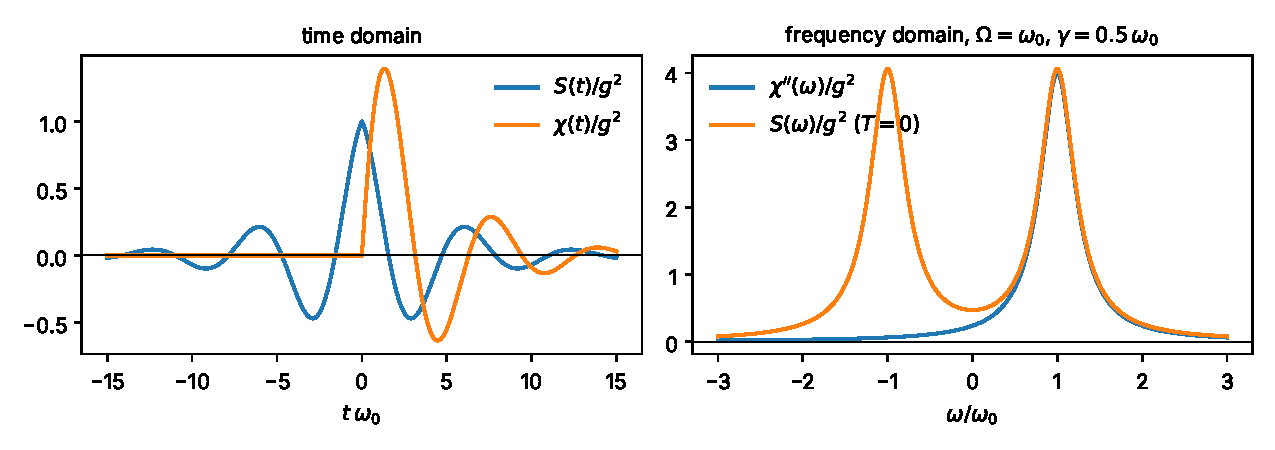
\includegraphics[width=\textwidth]{figures/fig_bath_kernels.pdf}
\caption{The Lorentzian bath used in the numerical examples. Left: noise kernel $S(t)$
(even in $t$) and response kernel $\chi(t)$ (causal, odd before the step function), from
\cref{eq:lorentz-kernels}. Right: $\chi''(\omega)$ and the zero-temperature noise spectrum
$S(\omega)=J(\omega)+J(-\omega)$. A $T_1$ measurement samples these at $\omega=\pm\omega_0$; a
dephasing measurement samples $S$ near $\omega=0$ (\cref{sec:lec10}).}
\label{fig:bath-kernels}
\end{figure}

\subsection{Why only $J(\omega)$ matters: Gaussianity and Wick's theorem}

The bath state is Gaussian (thermal state of a quadratic Hamiltonian) and $B$ is linear
in the $b_k$. Hence all higher moments of $B$ factorize into products of two-point
functions:
\begin{equation}
  \avg{T_{\mathcal C}\,B(z_1)B(z_2)\cdots B(z_{2n})}=\sum_{\text{pairings}}\ \prod_{\text{pairs }(ij)}\avg{T_{\mathcal C}\,B(z_i)B(z_j)},
  \qquad \avg{T_{\mathcal C}\,B(z_1)\cdots B(z_{2n+1})}=0 ,
  \label{eq:wick}
\end{equation}
for any ordering prescription $T_{\mathcal C}$ that is applied consistently inside each pair
(Wick's theorem; see~\cite[Sec.~2.5]{Kamenev2011} for the contour version). Since the
two-point function is built from $J(\omega)$ and $\beta$ alone, so is everything the system
can feel. This is the precise sense in which ``the bath is characterized by its spectral
density''. Non-Gaussian baths (spins, anharmonic modes, fermionic reservoirs with
interactions) need higher cumulants; the formalism of the following lectures survives
with pairings replaced by cumulants~\cite{Schoeller2009}, but we will not need this.

A useful way to say the same thing: for a Gaussian bath, a \emph{linear} coupling, and a
factorized initial state, the reduced dynamics of the system depends on the bath only
through $C(t)$. Any two baths with the same $C(t)$ produce identical $\rhoS(t)$. This is
the basis of the exact reference solution used in the numerics:

\begin{keybox}[The pseudomode mapping (Garraway~\cite{Garraway1997}; Tamascelli \emph{et al.}~\cite{Tamascelli2018})]
Consider the qubit coupled to a \emph{single} oscillator $a$ of frequency $\Omega$, which is
itself damped at rate $\gamma$ by a Markovian environment:
\begin{equation}
  \dot\rho=-i\big[H_S+\Omega a^\dagger a+g\,S\otimes(a+a^\dagger),\rho\big]
  +\gamma\big(a\rho a^\dagger-\tfrac12\{a^\dagger a,\rho\}\big),\qquad \rho(0)=\rhoS(0)\otimes\ket0\bra0 .
  \label{eq:pseudomode}
\end{equation}
The ``bath'' $B_{\rm pm}=g(a+a^\dagger)$ seen by the qubit is Gaussian with
$\avg{B_{\rm pm}(t)B_{\rm pm}(0)}=g^2\ee^{-i\Omega t-\gamma|t|/2}$, which is exactly the Lorentzian
$C(t)$ of \cref{eq:lorentz-kernels}. Therefore the qubit's reduced dynamics in
\cref{eq:pseudomode} is \emph{identical}, to all orders in $g$ and for all times, to its
dynamics in the full Lorentzian bosonic bath. The small Hilbert space (qubit $\otimes$ a
few oscillator levels) makes \cref{eq:pseudomode} trivially solvable numerically. The
price is the negative-frequency tail of $J$; the reward is an exact benchmark for every
approximation in these notes.
\end{keybox}

\subsection{Initial state and pictures}

We take $\rho(0)=\rhoS(0)\otimes\rhoB$ with $\rhoB$ thermal (so $[H_B,\rhoB]=0$ and
$\avg{B}=0$). Physically this means the coupling is switched on at $t=0$, or that the
qubit was prepared by a fast operation that does not disturb the bath. Correlated initial
states (for example the global thermal state of $H$) can be handled, at the price of an
inhomogeneous term in the master equation (\cref{sec:lec5}) or an imaginary-time branch
of the contour (\cref{sec:lec9}).

We will move freely between the Schr\"odinger picture, the interaction picture with
respect to $H_0=H_S+H_B$, and the Heisenberg picture. For the record, in the interaction
picture
\begin{equation}
  \tilde S(t)=\ee^{iH_St}S\ee^{-iH_St}=\cos\theta\,\sz+\sin\theta\big(\sx\cos\omega_0t-\sy\sin\omega_0t\big)
  =\cos\theta\,\sz+\sin\theta\big(\sigma_+\ee^{i\omega_0t}+\sigma_-\ee^{-i\omega_0t}\big),
  \label{eq:S-int}
\end{equation}
with $\sigma_\pm=\tfrac12(\sx\pm i\sy)$. Note that the Heisenberg-picture rotation of $\sx$ is
clockwise, opposite to the Schr\"odinger-picture rotation of the Bloch vector in
\cref{eq:LS-bloch}, as it must be. The $\cos\theta$ part is static, the $\sin\theta$
part oscillates at $\pm\omega_0$: this is why dephasing samples the bath at $\omega\approx0$ and
relaxation samples it at $\omega=\pm\omega_0$.

\subsection{Exercises}

\begin{exercise}\label{ex:2-1}
Derive \cref{eq:C} and check the single-mode case $J(\omega)=\pi g^2\delta(\omega-\omega_b)$ against
$S(t)=g^2(2\bar n+1)\cos\omega_bt$, $\chi(t)=2g^2\theta(t)\sin\omega_bt$. Verify \cref{eq:FDT} for this case.
\end{exercise}

\begin{exercise}\label{ex:2-2}
Prove $\chi''(\omega)=\sgn(\omega)J(|\omega|)$ from \cref{eq:chi-def} and derive the Ohmic kernels
of Example~2.1 at $T=0$. Then show that at finite $T$ and $\omega_c\to\infty$,
$S(t)\to-2\alpha(\pi T)^2/\sinh^2(\pi Tt)$ for $t\ne0$, and explain how a positive-definite
$S(\omega)$ can have a negative $S(t)$ at all $t>0$.
\end{exercise}

\begin{exercise}\label{ex:2-3}
Show that in \cref{eq:pseudomode} the oscillator's two-point function in the absence of
the qubit is $\avg{a(t)a^\dagger(0)}=\ee^{-(i\Omega+\gamma/2)t}$ for $t>0$ (use the quantum
regression theorem, or solve the adjoint equation for $a$), and that the state remains
Gaussian. This is the content of the pseudomode theorem; see~\cite{Tamascelli2018} for
the general statement.
\end{exercise}

\begin{exercise}\label{ex:2-4}
Verify the unitary equivalence \cref{eq:leggett-form}, and show that a bath coupled to
$S=\cos\theta\sz+\sin\theta\sx$ with correlation $C(t)$ is equivalent to \emph{two independent}
baths coupled to $\sz$ and $\sx$ only if the cross-correlation $\cos\theta\sin\theta\,C(t)$ is
dropped. We will see in \cref{sec:lec5} where this cross term goes.
\end{exercise}

\clearpage
